\documentclass[10pt]{beamer}

\usetheme{CambridgeUS}
\usepackage[english, russian]{babel}
\usepackage[utf8]{inputenc}
\usepackage{caption}
\usepackage{etoolbox}
\usepackage{multicol}
\usepackage{listings}
\usepackage{wasysym}
\usepackage{mathtools}
\DeclarePairedDelimiter\ceil{\lceil}{\rceil}
\DeclarePairedDelimiter\floor{\lfloor}{\rfloor}

\definecolor{mygreen}{rgb}{0,0.6,0}
\lstset{
  basicstyle=\ttfamily\footnotesize,        % the size of the fonts that are used for the code
  breaklines=true,                 % automatic line breaking only at whitespace
  captionpos=b,                    % sets the caption-position to bottom
  commentstyle=\color{mygreen},    % comment style
  keywordstyle=\color{blue},       % keyword style
  stringstyle=\color{red},     % string literal style
  showstringspaces=false,
  morekeywords={include, printf},
  texcl=true     %<---- added
}


\title[\href{https://goo.gl/NRgp8K}{https://goo.gl/NRgp8K} (Term 1)]{MST}
\author[Гусев Илья, Булгаков Илья]{Гусев Илья, Булгаков Илья}
\institute[МФТИ] 
{Московский физико-технический институт\\*}
\date{Москва, 2019}
\subject{Computer Science}

\begin{document}

\begin{frame}
  \titlepage
\end{frame}

\begin{frame}{Содержание}
\tableofcontents
\end{frame}

\section{Минимальное остовное дерево}

\begin{frame}[fragile]{Минимальное остовное дерево}



\begin{itemize}
    \item Остовное дерево - ациклический связный подграф данного связного неориентированного графа, в который входят все его вершины.
    \item Минимальное остовное дерево - остовное дерево минимального веса
\end{itemize}

\begin{center}
    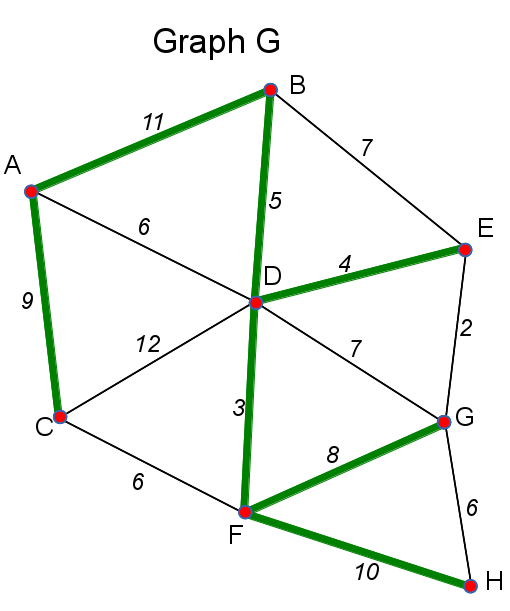
\includegraphics[width=4cm]{Term_2/Source/images/mst.png}
\end{center}

\end{frame}



\begin{frame}[fragile]{Минимальное остовное дерево}

Алгоритмы для построения
\begin{itemize}
    \item Алгоритм Прима (повторение алгоритма Дейкстры)
    \item Алгоритм Краскала
    \item Алгоритм Борувки
\end{itemize}

\end{frame}

\begin{frame}[fragile]{Лемма о безопасном ребре}
Рассмотрим связный неориентированный взвешенный граф $G=(V,E)$. Пусть $G^1=(V,E^1)$ — подграф некоторого минимального остовного дерева $G$, $<S,T>$ — разрез $G$, такой, что ни одно ребро из $E^1$ не пересекает разрез, а $(u,v)$ — ребро минимального веса среди всех ребер, пересекающих разрез $<S,T>$. Тогда ребро $e=(u,v)$ является безопасным для $G^1$.
\begin{center}
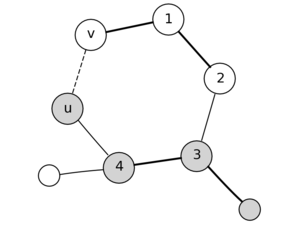
\includegraphics[height=4cm]{Term_2/Source/images/safe_lemma.png}
\end{center}
\end{frame}

\section{Алгоритм Прима}
\begin{frame}[fragile]{Алгоритм Прима}
Выбираем всегда кратчайшее ребро из соседних к уже построенному поддереву
\begin{center}
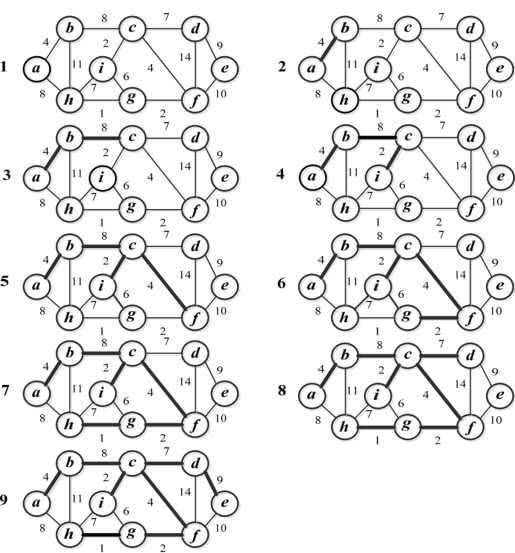
\includegraphics[height=6.5cm]{Term_2/Source/images/prim.png}
\end{center}
\end{frame}

\begin{frame}[fragile]{Алгоритм Прима}
Ничего не напоминает?

Какая асимптотика?
\end{frame}

\section{Алгоритм Крускала}
\begin{frame}[fragile]{Алгоритм Крускала}
\begin{itemize}
    \item Сортировка всех рёбер по весу
    \item На каждом шаге берём минимальное, которое не образует цикл
\end{itemize}
\begin{center}
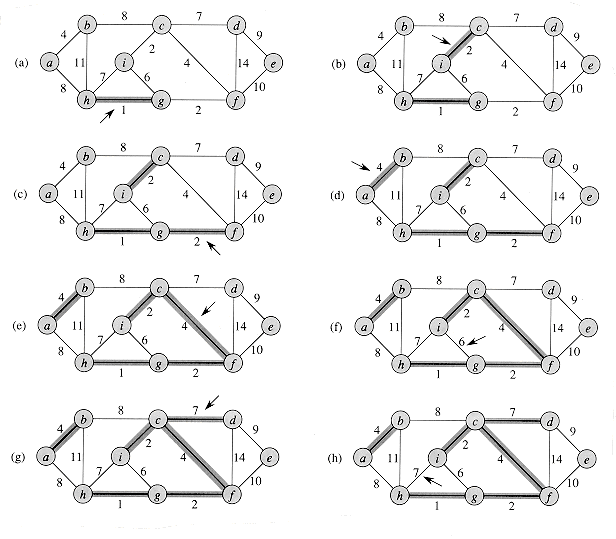
\includegraphics[height=6.5cm]{Term_2/Source/images/kruskal.png}
\end{center}
\end{frame}

\begin{frame}[fragile]{Алгоритм Крускала}
\begin{itemize}
    \item Наивная реализация: $O(E \cdot log(E) + E + V^2)$
    \item СНМ: $O(E \cdot log(E) + E + V)$
\end{itemize}
\end{frame}

\section{Система непесекающихся множеств}

\begin{frame}[fragile]{Система непесекающихся множеств}

Структура, поддерживающая операции над множествами: объединить два множества; проверить, в каком множестве элемент.
Английское название — disjoint set union (DSU)

\begin{itemize}
    \item {\rm make\_set}(x) — добавляет новый элемент x, помещая его в новое множество, состоящее из одного него.
    \item {\rm union\_sets}(x,y) — объединяет два указанных множества (множество, в котором находится элемент x, и множество, в котором находится элемент y).
    \item {\rm find\_set}(x) — возвращает, в каком множестве находится указанный элемент x. На самом деле при этом возвращается один из элементов множества (называемый представителем или лидером (в англоязычной литературе "leader")). Этот представитель выбирается в каждом множестве самой структурой данных (и может меняться с течением времени, а именно, после вызовов {\rm union\_sets}())
\end{itemize}

\end{frame}

\begin{frame}[fragile]{Система непесекающихся множеств}

Наивная реализация. Каждое множество храним в виде дерева. Используем массив parent - для каждого элемента храним родителя.

\begin{lstlisting}
vector<int> parent(elementsCount);

void make_set (int v) {
	parent[v] = v;
}
 
int find_set (int v) {
	if (v == parent[v])
		return v;
	return find_set (parent[v]);
}
 
void union_sets (int a, int b) {
	a = find_set (a);
	b = find_set (b);
	if (a != b)
		parent[b] = a;
}
\end{lstlisting}
\end{frame}

\begin{frame}[fragile]{Система непесекающихся множеств. Оптимизации}

Эвристика сжатия пути

\begin{lstlisting}

int find_set (int v) {
	if (v == parent[v])
		return v;
	return parent[v] = find_set (parent[v]);
}
\end{lstlisting}
\end{frame}

\begin{frame}[fragile]{Система непесекающихся множеств. Оптимизации}

Эвристика объединения по рангу или размеру дерева. Заводим дополнительный массив size, который хранит число вершин в поддереве (есть модификация с глубиной дерева)

\begin{lstlisting}

vector<int> size(elementsCount);

void union_sets (int a, int b) {
	a = find_set (a);
	b = find_set (b);
	if (a != b) {
		if (size[a] < size[b])
			swap (a, b);
		parent[b] = a;
		size[a] += size[b];
	}
}

\end{lstlisting}
\end{frame}

\begin{frame}[fragile]{Система непесекающихся множеств. Сложность}

Время работы

\begin{itemize}
    \item Наивный - может вырожиться в цепочку вплоть до O(n)
    \item Использование одной из эвристик дает среднее время O(log n)
    \item Использование обоих эвристик дает среднее время O(1)
\end{itemize}

\end{frame}

\section{Задача коммивояжёра}
\begin{frame}[fragile]{Задача коммивояжёра}
\begin{itemize}
    \item Задача коммивояжёра — нахождение мнимального пути между городами с посещением каждого города ровно один раз.
    \item Решение задачи коммивояжёра — это нахождение гамильтонова цикла минимального веса.
\end{itemize}
\end{frame}

\begin{frame}[fragile]{Задача коммивояжёра}
Ограничения:
\begin{itemize}
    \item Полностью связный граф
    \item Используем метрическую постанвку: выполняется неравенство треугольника
\end{itemize}
\end{frame}

\begin{frame}[fragile]{Задача коммивояжёра и MST}
\begin{center}
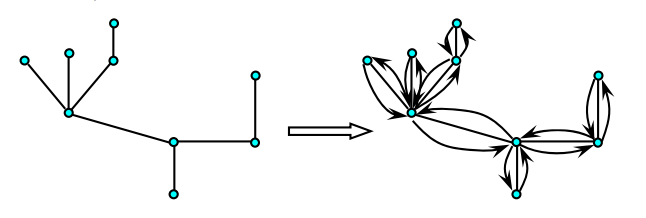
\includegraphics[height=3cm]{Term_2/Source/images/kom1.png}
\end{center}
\begin{center}
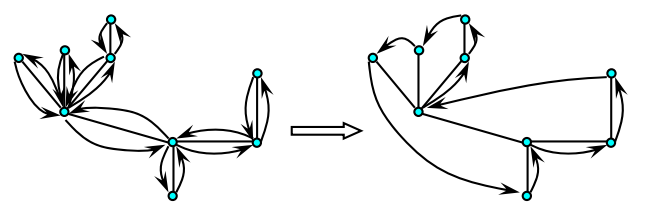
\includegraphics[height=3cm]{Term_2/Source/images/kom2.png}
\end{center}
\end{frame}

\appendix

\begin{frame}[allowframebreaks]
  \frametitle<presentation>{Полезные ссылки}
    
  \begin{thebibliography}{10}
{
  \beamertemplatebookbibitems
  % Start with overview books.
  
  \bibitem{ran}
 \texttt{Задача коммивояжера - Институт математики СО РАН}
  \newblock \href{http://www.math.nsc.ru/LBRT/k5/OR-MMF/TSPr.pdf}{\texttt{http://www.math.nsc.ru/LBRT/k5/OR-MMF/TSPr.pdf}}
    
  \bibitem{neerc}
  \texttt{Викиконспекты: лемма о безопасном пути}
  \newblock \href{https://bit.ly/2YIlQvk}{\texttt{https://bit.ly/2YIlQvk}}
  
  \bibitem{neerc}
  \texttt{Викиконспекты: лемма о безопасном пути}
  \newblock \href{https://bit.ly/2YIlQvk}{\texttt{https://bit.ly/2YIlQvk}}
 
}
  \end{thebibliography}
  \end{frame}

\end{document}


